\documentclass[12pt]{article}
\oddsidemargin=0.0in
\evensidemargin=0.0in
\textwidth=6.5in
\topmargin=-0.75in
\textheight=9.5in
\usepackage{hyperref}
%\usepackage{url}
\usepackage{graphicx}
\usepackage{amsmath}

\begin{document}
\pagestyle{empty}
 
\begin{center}
{\LARGE {\bf Homework Eight}}\\
\bigskip
{\Large {\bf Calculus I}}\\
\bigskip
{\Large {\bf College of the Atlantic}}\\
\bigskip
{ {\bf Due Friday, November 8, 2024}}\\ 
\end{center}
\medskip

%\noindent There are two parts to this assignment.\\

\noindent {\bf Part 1: WeBWorK}.  Do Homework 08A on
WeBWorK.  The WeBWorK page is here:
\url{https://webwork-hosting.runestone.academy/webwork2/coa-feldman-es1024-fall2024}
I recommend doing the WeBWorK part of the homework first.  This will
enable you to benefit WeBWorK's instant feedback before you do part
two.\\ 


\noindent {\bf Part 2: Non-WeBWorK problems}.  Here are some
instructions for how to submit this part of the assignment.
\begin{itemize}
  \setlength{\itemsep}{0mm}
\item Do the problems by hand using pencil (or pen) and paper.
  There is no need to type this assignment.
%\item If you like working on a tablet, go for it. 
\item Make a pdf scan of your work using genius scan or some
  similar scanning app.  Please make the homework into a single
  pdf, not multiple pdfs.
\item Submit the assignment on google classroom.  Please don't
  email it to me.
  %(Between my two classes I will be receiving
  %around 60 assignments a week.  Keeping track of them all in email 
  %is challenging.)
%\item If you want, you can do the non-WeBWorK problems in pairs and
%  submit only one assignment for the two of you. 
\end{itemize}

\noindent Here are some non-WeBWorK problems.


\begin{enumerate}
\setlength{\itemsep}{3mm}


\item Consider the function $g(x) = xe^x$.
\begin{enumerate}
\setlength{\itemsep}{-1mm}
  \item Find exact values for and classify all critical
    points. Determine any local maxima or minima ($x$ and $y$ values). 
  \item Find exact values for  all inflection points.  
  \item Sketch the function.
\end{enumerate}

\item Consider the function $h(x) = x + \sin(x)$.  
\begin{enumerate}
\setlength{\itemsep}{-1mm}
  \item Find exact values for and classify all critical
    points. Determine any local maxima or minima ($x$ and $y$ values).  
  \item Find exact values for  all inflection points.  
  \item Sketch the function.
  \item Explain in a few sentences why the function has the shape that
    it does.  
\end{enumerate}

\item Figure \ref{fig:birds} shows how the rate $f(v)$ at which a bird
  uses energy to fly (measured in Joules/s) depends on the speed of
  the bird (measured in m/s).  Let $a(v)$ be the amount of energy
  consumed by the same bird, measured in Joules/m.
  \begin{enumerate}
    \setlength{\itemsep}{0mm}
  \item What is the relationship between $f(v)$ and $a(v)$?
  \item At what speed is $f(v)$ minimized? (Show the value on the graph.)
  \item At what speed is $a(v)$ minimized? (Show the value on the graph.)
  \item Under what circumstances might a bird want to fly so as to
    minimize $f(v)$?
    \item Under what circumstances might a bird want to fly so as to
      minimize $a(v)$?
  \end{enumerate}

  
\begin{figure}[h!]
\begin{center}
\vspace{-1mm}
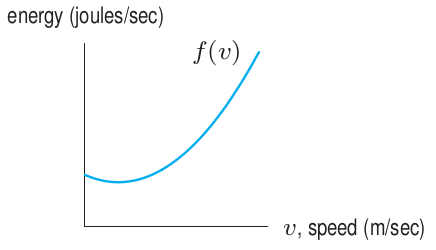
\includegraphics[width=6.7in]{birds.png}
\vspace{-2mm}
\caption{The amount of energy used by a flying bird.}
\label{fig:birds}
\vspace{9mm}
\end{center}
\end{figure}


%\item A bird gathers worms to feed to its young.  To do so, it flies
%  from its nest to wherever the worms are, picks up several worms in
%  its beak, and then returns to its nest to feed its hungry
%  children. A \emph{loading curve}, such as the one shown in
%  Fig.~\ref{fig:worms}, shows how the number of worms the bird picks
%  up depends on the time the bird spends searching.
%  \begin{enumerate}
%    \setlength{\itemsep}{1mm}
%  \item Why might the shape of the curve be concave down?  
%  \item The time it takes the bird to travel from its next to the
%    worm-gathering place is represented by the distance PO in
%    Fig.~\ref{fig:worms}.  The birds (and its young) want to maximize
%    the rate it which it brings worms to the next. This quantity is
%    given by:
%    \begin{equation}
%      \text{Rate Worms Arrive} \, = \, \frac{\text{Number of
%          Worms}}{\text{Traveling time} + \text{Searching time}} \;.
%    \end{equation}
%    \item Draw a line on Fig.~\ref{fig:worms} whose slope is equal to
%      the rate at which worms arrive.
%    \item Using the figure, estimate the load (number of worms) which
%      maximizes the worm arrival rate.
%    \item If the traveling time is increased, does the optimal load
%      increase or decrease?  Why?
%  \end{enumerate}


%\begin{figure}[h!]
%\begin{center}
%\vspace{-1mm}
%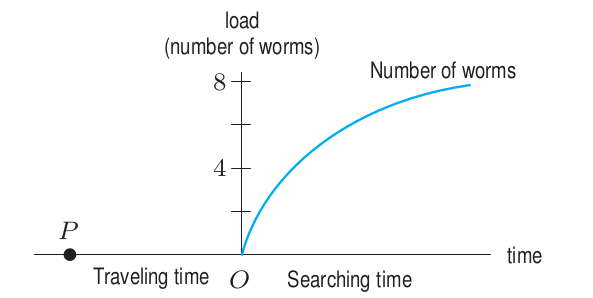
\includegraphics[width=5.60in]{worms.png}
%\vspace{-2mm}
%\caption{The load curve for the worm-gathering bird.}
%\label{fig:worms}
%\vspace{-5mm}
%\end{center}
%\end{figure}

%\item The cost of fuel (in dollars per hour) needed to move a boat
%  through the water is proportional to the cube of the speed.  (This
%  means that $C=kv^3$.)  A ferry boat uses \$100 of fuel per hour if
%  it is cruising at 10 km per hour.  The fuel isn't the only cost for
%  the ferry. You also need to pay the crew. This cost comes to \$675
%  per hour. At what speed should the ferry travel so as to minimize
%  the cost per kilometer traveled? 


\item A ball is thrown straight up from the top of a $30$ meter
  building. The initial speed of the ball is $v_0$.  The height of the
  ball as a function of time is given by:
\begin{equation}
  y \, = \, -10t^2 + v_0 t + 30 \;.
\end{equation}
\begin{enumerate}
%\setlength{\itemsep}{0mm}
  \item At what time does the ball reach its highest point?
  \item What is the maximum height reached by the ball?
  \item How fast must the ball be thrown so that it makes it $100$
    meters above the ground?
\end{enumerate}


\end{enumerate}

\end{document}




  \item Determine an equation for the linear function that generates
    the values in the table below.  

\begin{center}
\begin{tabular}{|| l | l ||}
\hline $x$ & $f(x)$ \\
\hline
5.2 & 27.8 \\
5.3 & 29.2 \\
5.4 & 30.6 \\
5.5 & 32.0 \\
5.6 & 33.4 \\
\hline
\end{tabular}
\end{center}





\end{document}
